\section{Konzept der Ereignisverarbeitung}\label{sec:Ereignisverarbeitung}
In der realen Welt ist eine Wechselwirkung aller Geschehnisse mit einer Vielzahl von divergenten, meist nicht-deterministisch eintretenden Ereignissen zu beobachten, als Konsequenz folgt eine signifikante Beeinflussung auf den Fortgang der Geschehnisse.
\cite{Grauer.2010}
Dieser Tatbestand findet sich auch in den Abläufen und Geschäftsprozessen in Unternehmen wieder.
Ein Unternehmen ist demzufolge gezwungen, auf diese Ereignisse angemessen und möglichst zeitnah zu reagieren – die Unternehmen operieren demnach ereignisgesteuert. 
\cite{Schaaf.2015}
Mit dem Konzept der Ereignisverarbeitung rücken Ereignisse als zentraler Leitgedanke einer Orientierung an Ereignissen in den Fokus der Gestaltung von Geschäftsprozessen, indem Ereignisse als Baustein der Softwarearchitektur und der Geschäftslogik in den Mittelpunkt der Betrachtung rücken. 
\cite{Bruns.2010}

Die resultierenden ereignisgesteuerten Unternehmensanwendungen ermöglichen eine praxisnahe Darstellung der dynamischen Geschäftsprozesse eines Unternehmens. 
Das Ziel ist es dadurch die Agilität, Reaktionsfähigkeit und Echtzeitfähigkeit der Geschäftsprozesse eines Unternehmens zu erhöhen. 
In der Praxis hat eine derartige Ereignisorientierung in Unternehmensanwendungen bereits breiten Zuspruch gefunden. 
\cite{Bruns.2015}
In diesem Kontext beruhen ereignisgesteuerte Architekturen, englisch \ac{EDA}, auf einem ereignisgesteuerten Prinzip, bei dem eine lose Kopplung zwischen den beteiligten Komponenten eines Informationssystems vorgesehen ist.  
In ihrer reinen Ausprägung kommunizieren diese Komponenten ausschließlich mittels sogenannter Ereignisbenachrichtigungen, englisch \textit{event messages}, miteinander.
Abbildung \ref{fig:Grundschritte von ereignisgesteuerten Architekturen} illustriert den Ablauf der Grundschritte ereignisgesteuerter Architekturen, deren Charakteristika nachfolgend erläutert werden.
\cite{Schaaf.2015}

\begin{figure}[H]
	\centering 
    \begin{tikzpicture}
        \fill[even odd rule, white] circle (1.5);
    
       \node at (0,0) [
          font  = \sffamily\Large\bfseries\color{black!85},
          align = center
       ]{
          \acs{EDA}
       };
       \arcarrow{197}{ 96}{Erkennen}
       \arcarrow{ 89}{-17}{Verarbeiten}
       \arcarrow{199}{341}{Reagieren}
    \end{tikzpicture}
    \caption[Grundschritte von ereignisgesteuerten Architekturen]
    {Grundschritte von ereignisgesteuerten Architekturen \protect\footnotemark}
    \label{fig:Grundschritte von ereignisgesteuerten Architekturen}
\end{figure}
\footnotetext{in Anlehnung an \citeauthor{Bruns.2010} \citeyear{Bruns.2010} \cite{Bruns.2010} }

Demnach besteht eine zentrale Charakteristik von ereignisgesteuerten Architekturen aus der Komposition von drei Grundschritten: \textit{Erkennen, Verarbeiten und Reagieren von oder auf Ereignisse.}

% \paragraph{Erkennen} 
Das Auftreten von relevanten Informationen und Sachverhalten in  den Geschäftsprozessen ist der Ausgangspunkt für die Erkennung von Ereignissen.
Diese Informationen und Sachverhalte werden analysiert, als Ereignisse klassifiziert und spiegeln einen spezifizierten Ausschnitt des Zustands eines Geschäftsprozesses wieder. 
Für registrierte Ereignisse wird ein entsprechendes Ereignisobjekt generiert.
Entscheidend für ereignisgesteuerte Informationssysteme ist, dass die Ereignisse unmittelbar zum Zeitpunkt ihres Auftretens erkannt werden und nicht zeitverzögert.
\cite{Bruns.2010}

% \paragraph{Verarbeiten}
Im Verarbeitungsschritt werden die erkannten Ereignisse, die aus unterschiedlichen Ereignisquellen stammen können, analysiert. Bei der Analyse werden Ereignisse mit anderen Ereignissen verknüft, generalisiert, aufgeteilt oder aber auch als irrelevant eingestuft. 
Gesucht werden Paradigmen in den gesammelten Ereignissen, die bestimmte Beziehungen und Abhängigkeiten zwischen den Ereignissen ausdrücken.
\cite{Hedtstuck.2017}

% \paragraph{Reagieren}
Aufgrund von identifizierten Ereignissobjekten, die im Fluss der eingetretenen Ereignisse erkannt wurden, können vielfältige Arten von Reaktionen zeitnah veranlasst werden.
Die Reaktionen, die angestrebt werden, charkterisieren sich durch Aktualität und Individualität, wie etwa die unmittelbare Übergabe der Ereignisse an Anwendungssysteme, das Senden von Benachrichtigungen, der Aufruf von Funktionen in Form von digitalen Diensten, das Auslösen eines Geschäftsprozesses oder die Initiierung von manuellen Aktivitäten durch menschliche Benutzer, aber auch die Generierung neuer Ereignisse ist eine legitime Reaktion.
\cite{Bruns.2010}

Im Zusammenhang mit der Ereignisverarbeitung in Unternehmensanwendungen wird der Begriff Echtzeit, englisch \textit{real-time}, häufig verwendet, um die Aktualität von verarbeiteten Ereignissen zu hervorzuheben.
\cite{Bruns.2015}
Echtzeit wird jedoch nicht im Sinne der Informatik verstanden, wonach für jede Funktion die exakte Einhaltung einer restriktiv vorgeschriebenen Antwortzeit erforderlich ist, um die Gegenwartsbezogenheit und Vorhersagbarkeit von Informationssystemen sicherzustellen.
Vielmehr dominiert ein betriebswirtschaftliches Verständnis, das darauf Bedacht ist, in allen relevanten Informationssystemen aktuelle Informationen bereitzustellen, ohne spezifizierte Leistungskennzahlen zur Erfüllung von Echtzeit zu formulieren.
\cite{Worn.2005}
Unter Echtzeit versteht man aus dieser Sicht daher die möglichst zeitnahe Verfügbarkeit, Transparenz und Nutzbarkeit von Informationen ohne unnötige Zeitverzögerung.
Eingehende Ereignisse werden somit im Rahmen der Ereignisverarbeitung analysiert, sobald sie auftreten, um geeignete Reaktionen in Echtzeit auslösen zu können.
\cite{Grauer.2010}

\subsection{Merkmale und Kriterien}
Der Austausch von Ereignissen in einer \ac{EDA} wird typischerweise durch das in Abbildung \ref{fig:Publish-Subscribe-Paradigma} dargestellte \textit{Publish-Subscribe-Paradigma} realisiert. 
Ein Produzent, englisch \textit{publisher}, sendet seine Ereignisse in Form von Ereignisobjekten an eine verarbeitende Schicht, um diese in sogenannten Ereigniskanälen kategorisiert zur Verfügung zu stellen. Die publizierten Ereignisobjekte sind Instanzen eines spezifischen Ereignisses.
\cite{Metz.2014}

\begin{figure}[H]
	\centering 
    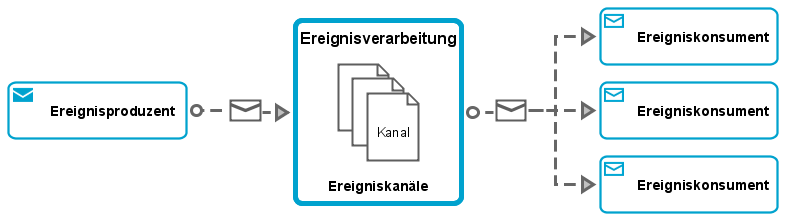
\includegraphics[width=\textwidth]{img/pubsub.png}	
    \caption[Publish-Subscribe-Paradigma]
    {Publish-Subscribe-Paradigma \protect\footnotemark}
    \label{fig:Publish-Subscribe-Paradigma}
\end{figure}
\footnotetext{in Anlehnung an \citeauthor{Metz.2014} \citeyear{Metz.2014} \cite{Metz.2014} }

Ein oder mehrere Konsumenten, englisch \textit{subscriber}, bekunden ihr Interesse an einem oder mehreren Ereigniskanälen, indem sie sich mittels der Ereignisverarbeitung für diesen Ereigniskanal oder diese Ereigniskanäle registrieren. 
Diese abonnieren somit die Zustellung aller Ereignisobjekte der registrierten Ereigniskanäle.
Beim Abonnieren ist es möglich, dass mehrere Empfänger an demselben Ereigniskanal interessiert sind, sodass sich sowohl eine 1:1- als auch eine 1:n-Kommunikation realisieren lässt. 
Beim Eintreffen eines neuen Ereignisobjekts benachrichtigt die Ereignisverarbeitung alle an dem zugehörigen Ereigniskanal interessierten Parteien über dessen Eintreffen. 
Jeder Empfänger kann das neue Ereignisobjekt zu einem von ihm bestimmten Zeitpunkt verarbeiten.
\cite{Schaaf.2015}
Das Publish/Subscribe-Paradigma führt zu einem entkoppelten Verarbeitungsmodell. Aus der entkoppelten Verarbeitung folgt aber gleichzeitig der Verlust einer deterministischen Reihenfolge der Verarbeitungsschritte.
\cite{Bruns.2010}

Die \ac{EDA} wird, wie schon erwähnt, im Wesentlichen durch die drei Grundschritte Erkennen, Verarbeiten und Reagieren charakterisiert, woraus sich drei logische architektonische Schichten für eine Ereignisverarbeitung ergeben: Ereignisquellen, Ereignisverarbeitung und Ereignisbehandlung. Das
Zusammenspiel dieser drei Schichten wird  in Abbildung \ref{fig:Grundlegender architektonischer Entwurf einer EDA} veranschaulicht.

\begin{figure}[H]
	\centering 
    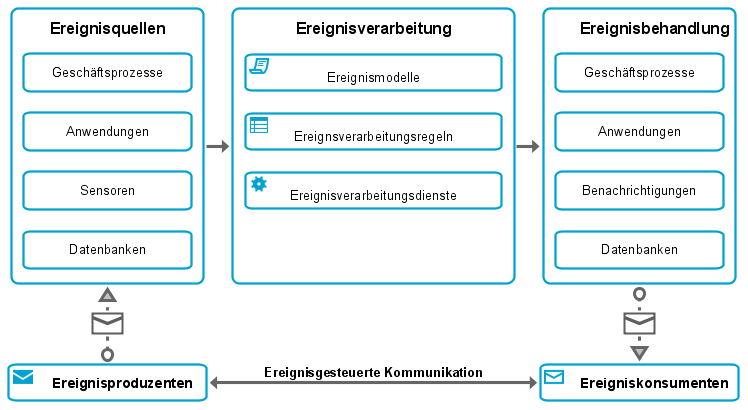
\includegraphics[width=\textwidth]{img/Ereignisverarbitungablauf.png}	
    \caption[Grundlegender architektonischer Entwurf einer EDA]
    {Grundlegender architektonischer Entwurf einer EDA \protect\footnotemark}
    \label{fig:Grundlegender architektonischer Entwurf einer EDA}
\end{figure}
\footnotetext{in Anlehnung an \citeauthor{Bruns.2010} \citeyear{Bruns.2010} \cite{Bruns.2010} }

Ein Ereignisproduzent, der relevante Sachverhalte und Informationen als Ereignisse erkennt und entsprechende Ereignisobjekte generiert, wird im Kontext von \ac{EDA} als Ereignisquelle bezeichnet.  
\cite{Bruns.2010}
Eine Ereignisquelle sendet eine Ereignisbenachrichtigung mit den Daten über das Auftreten eines Ereignisses an die Ereignisverarbeitung. 
Die Ereignisquelle leitet hierbei das Ereignis als Ereignisbenachrichtigung an die Verarbeitungsschicht weiter, ohne zu wissen, wo und wie das Ereignis weiterverarbeitet wird. 
Allein die Ereignisverarbeitung ist verantwortlich für die fehlerfreie Verteilung der Ereignisbenachrichtigungen und verfügt über das entsprechende Wissen. 
Auch die Verfügbarkeit oder überhaupt die Existenz einer weiterverarbeitenden Komponente ist der Quelle nicht bekannt. 
\cite{Bruns.2010}
Die Ereignisquelle bestimmt den Zeitpunkt des Sendens. 
Durch das aktive Senden eines Ereignisses unmittelbar zu dem Zeitpunkt, an dem es erkannt wird, reduziert sich die Zeit, um auf ein Ereignis zu reagieren. 
Als Konsequenz besitzen EDAs eine äußerst hohe Aktualität.
In welcher Weise die Ereignisobjekte an die weiterverarbeitende Schicht gelangen, hängt von den eingesetzten Technologien und den Möglichkeiten der Ereignisquellen ab.
\cite{Hedtstuck.2017}

Die eigentliche Verarbeitung der ankommenden Ereignisse erfolgt durch die Ereignisverarbeitung. 
Die fachliche Logik zur Behandlung von Ereignisobjekten ist in Form von deklarativen Ereignisregeln modelliert und definiert Aktionen, die auszuführen sind. 
Im Ereignismodell werden die in Betracht kommenden Eigenschaften, Verbindungen und Abhängigkeiten von Ereignissen konkretisiert. Im Sinne einer losen Kopplung muss jedes Ereignis alle für die Verarbeitung notwendigen Daten implizieren. Dazu gehören sowohl Metadaten wie Typ, Quelle und Auftrittszeitpunkt eines Ereignisses als auch die eigentlichen Betriebsdaten.
\cite{Bruns.2010}
Die eigentliche Ereignisbehandlung als Reaktion auf Ereignisobjekt erfolgt in den Anwendungssystemen nachgelagerten Ereignisverarbeitungsdiensten. 
Das Anwendungssystem selbst realisiert den Geschäftsprozess oder die digitalen Dienste, die von den Ereignissen angestoßen werden. 
\cite{Muhl.2006}

\subsection{Bewertung der Eignung von Ereignisverarbeitung}
Insbesondere im Hinblick auf die Erfordernisse beim Echtzeitmanagement von Betriebsdaten, immer schneller und mit hoher Dynamik auf Ereignisse im Geschäftsumfeld reagieren zu können, verspricht der Ansatz der Ereignisverarbeitung großes Potenzial.
Die unverzügliche Behandlung von Ereignissen, die Identifikation von Verknüpfungen aus einer Reihe von Ereignissen sowie die sich Nutzen bringend einordnende \ac{EDA}, machen die Ereignisverarbeitung zu einer adäquaten Möglichkeit zur Unterstützung von Echtzeitmanagement.
\cite{Vidackovic.2010} 

Auch wenn die technologischen Möglichkeiten als gegeben angesehen werden können, mangelt es dem Konzept der Ereignisverarbeitung für den praktischen Einsatz dennoch an Standards bei Ereignismodellen und Ereignisverarbeitungsdiensten sowie an grundsätzlichen Vorgehensweisen und dem unverzichtbaren Erfahrungswissen. 
\cite{Etzion.2011}
In der Realität existieren des Weiteren kaum Geschäftsprozesse, bei denen eine ausschließliche Kommunikation mithilfe von Ereignissen und ausschließlich im Rahmen der beschriebenen Grundschritte einer \ac{EDA} erfolgen, weshalb auch Anwendungssysteme mit teilweiser Ereignisverarbeitung und partieller Anwendung dieser Grundschritte die Umsetzung einer ereignisgesteuerten Architektur zugeschrieben.
\cite{Etzion.2011}


Um in diesem Kontext den betrachteten Defiziten angemessen begegnen zu können, intendiert die vorliegende Bachelorarbeit eine durchaus etablierte Ausprägung der \ac{EDA} als Komplement einer \ac{SOA}.
Die \ac{SOA}-Architektur beinhaltet, wie in Abschnitt \ref{sec:Automatisierung} beschrieben, die Konzepte, die notwendig sind, um Echtzeitmanagement zu ermöglichen und die Unterstützung der Dynamik ereignisgesteuerter Geschäftsprozesse zur selben Zeit zu gewährleisten, nicht vollständig.
Eine \ac{SOA} ohne Ereignisverarbeitung ist folglich nicht in der Lage, den aktuellen Zustand von Aktivitäten zu erkennen, da hierzu in Echtzeit temporale und kausale Verbindungen zwischen Geschäftsprozessen und Aktivitäten identifiziert und analysiert werden müssen. 
Eine \ac{EDA} kann als Maßnahme demnach eine \ac{SOA} komplementieren, zumal beide Konzepte grundsätzlich modulare und verteilte Informationssysteme mit loser Kopplung unterstützen, um durch die Nutzung der beiden Architekturen im Kollektiv zu profitieren. 
Für diese Kombination von \ac{SOA} und \ac{EDA} wird in der Literatur auch die Bezeichnung Event-Driven SOA genutzt. \todo{Durch SOEDA ersetzen}
\cite{Bruns.2010}
In dieser Ausprägung können Ereignisse den Aufruf von digitalen Diensten auslösen, woraufhin im Verlauf, deren Ausführung weitere Ereignisse generiert werden, die parallel von einem Ereignisverarbeitungsdienst analysiert und verarbeitet werden. 
\cite{Bruns.2010}